\begin{figure}[!tb]
  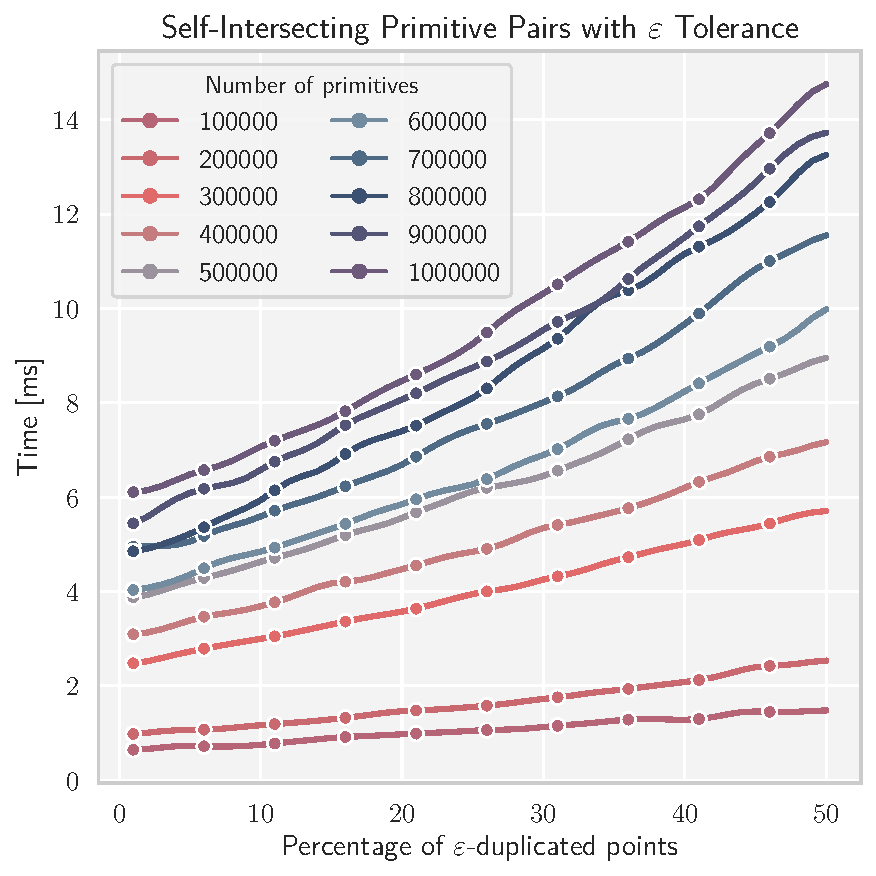
\includegraphics[width=\linewidth]{../figures/self_search_matrix.pdf}
\caption{
Performance of \texttt{tf::tree} on detecting $\varepsilon$-self-intersections.
Each curve corresponds to a point cloud of fixed size, with the x-axis indicating
the percentage of points duplicated and displaced by $\varepsilon$. The results
show that \texttt{tf::tree} maintains interactive self-query times even under
growing redundancy and scale.
}
\label{fig:self-search}
\end{figure}
